\section{Modern C++ in \odeint}

\begin{frame}

\heading{Modern C++ in \odeint}

\vspace{4ex}

\begin{itemize}
\item Iterators
\end{itemize}
\begin{itemize}
\item Using CUDA / OpenCL (Separation of algorithm from arithmetics)
\end{itemize}


\end{frame}






\begin{frame}[fragile]

\heading{ODEs are solve iteratively}

\vspace{3ex}
Constant step size integration:
\begin{lstlisting}
integrate_const(rk4, ode, x, t1, t2, dt,
  []( const state_type &x , double t ) {
    cout << x[0] << " " << x[1] << "n"; } );
\end{lstlisting}

\vspace{1ex}
Adaptive step size integration:
\begin{lstlisting}
integrate_adaptive(dopri5, ode, x, t1, t2, dt,
  []( const state_type &x , double t ) {
    cout << x[0] << " " << x[1] << "n"; } );
\end{lstlisting}

\vspace{2ex}
\centerline{\bf Can one use iterators?}

\end{frame}




\begin{frame}[fragile]

\heading{Iterators}

\vspace{2ex}

Iterators
\begin{lstlisting}[basicstyle=\tiny\ttfamily]
auto first = make_const_step_iterator_begin(rk4, ode, x, t1, t2, dt );
auto last = make_const_step_iterator_end(rk4, ode, x );
\end{lstlisting}

\vspace{2ex}

Ranges
\begin{lstlisting}[basicstyle=\tiny\ttfamily]
auto r = make_const_step_range(rk4, ode, x, t1, t2, dt );
\end{lstlisting}




\vspace{2ex}

{\small
\begin{itemize}
\item odeint's iterators are single-pass iterators
\item Specializations for stepper concepts
\item {\tt const\_step\_iterator<>}, {\tt adaptive\_iterator<>}
\item {\tt const\_step\_time\_iterator<>}, {\tt adaptive\_time\_iterator<>} -- value type is a pair of state and time of the ODE
\end{itemize}
}

\rem{
\begin{lstlisting}[basicstyle=\tiny\ttfamily]
template< class Stepper , class System >
class const_step_iterator : public boost::iterator_facade <
    const_step_iterator< Stepper , System > ,
    typename Stepper::state_type const ,
    boost::single_pass_traversal_tag >
{
    ...
};
\end{lstlisting}
}


\end{frame}






\begin{frame}[fragile]

\heading{Do fancy stuff with iterators!}

\vspace{2ex}

Average of the $x$-component of the solution
\begin{lstlisting}[basicstyle=\footnotesize\ttfamily]
double av = boost::accumulate(
  make_const_step_range(rk4, ode, x, t1, t2, dt),
  0.0, []( double sum , const state_type &x ) {
      return sum + x[0]; } );
\end{lstlisting}

\vspace{2ex}

Find the first occurence of a threshold
\begin{lstlisting}[basicstyle=\footnotesize\ttfamily]
auto iter = boost::find_if(
  make_const_step_time_range(rk4,ode, x, t1, t2, dt),
    [](const std::pair< state_type &, double> &x) {
      return ( x.first[0] < 0.0 ); } );
\end{lstlisting}


\end{frame}






\begin{frame}

\heading{CUDA/OpenCL for solving large system}

\vspace{2ex}

\begin{minipage}{0.48\textwidth} \begin{center}
  Lattice systems

  \vspace{3ex}

  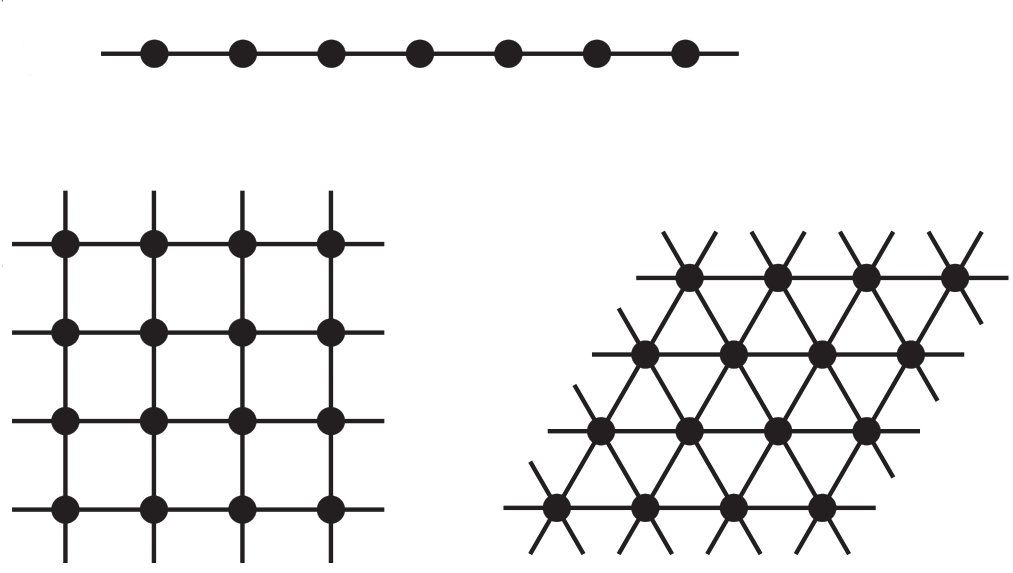
\includegraphics[draft=false,width=0.8\textwidth]{lattices.jpg}
\end{center} \end{minipage}
%\pause
\begin{minipage}{0.48\textwidth} \begin{center}
  Discretiztations of PDEs

  \vspace{0.5ex}
  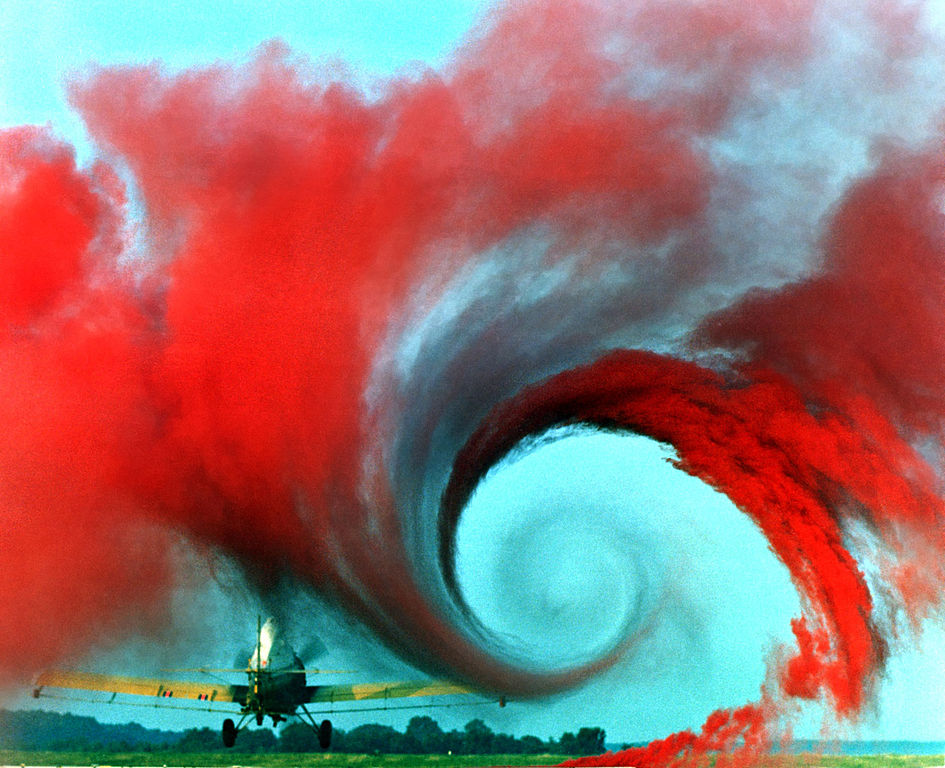
\includegraphics[draft=false,width=0.7\textwidth]{turbulence.jpg}
\end{center} \end{minipage}

%\pause
\vspace{2ex}

\begin{minipage}{0.48\textwidth}\begin{center}
  ODEs on graphs

  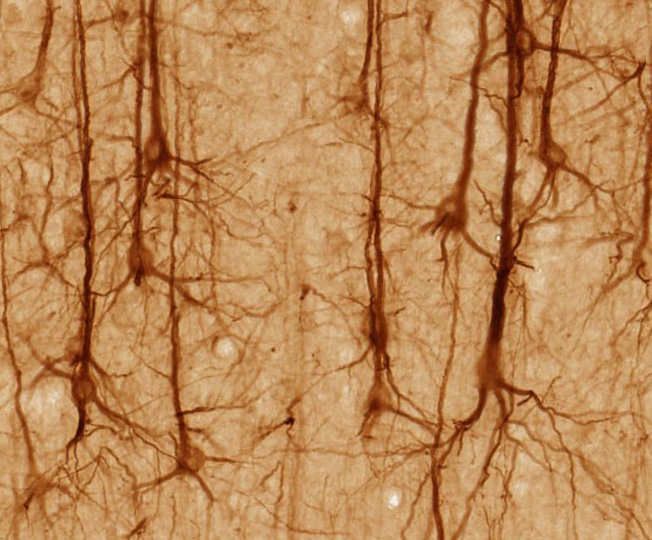
\includegraphics[draft=false,width=0.7\textwidth]{neuron.jpg}
 \end{center}\end{minipage}%\pause
\begin{minipage}{0.48\textwidth}\begin{center}
  Parameter studies
 
  \vspace{0.5ex}
  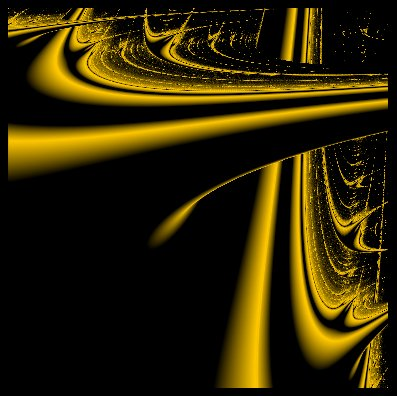
\includegraphics[draft=false,width=0.59\textwidth]{lyap.jpg}
 \end{center} \end{minipage}



\end{frame}







\begin{frame}[fragile]
 
\heading{Nonlinear pendulum -- Deterministic chaos}

 $$
  \dot{x} = y \quad \quad \dot{y} = - \sin(x) - \mu y + \varepsilon \sin \omega_E t 
 $$

\vspace{2ex}
Perturbations grow exponentially fast -- Butterfly effect

\vspace{3ex}
\begin{minipage}{0.48\textwidth} \begin{center}
\centerline{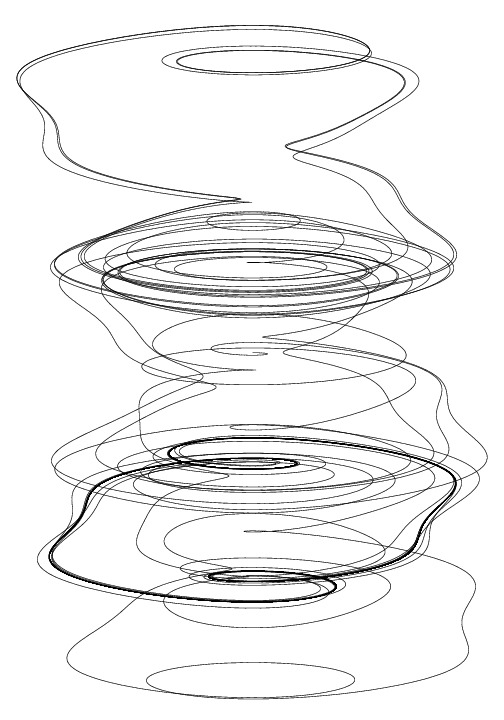
\includegraphics[draft=false,angle=270,width=1.0\textwidth]{pendulum2.jpg}}
\end{center}\end{minipage}\begin{minipage}{0.48\textwidth}\begin{center}
Does one observe chaos over the whole parameter range?

\vspace{2ex}
Vary $\varepsilon$ from $0$ to $5.0$ and $\omega_E$ from $0.5$ to $1.5$ and determine chaoticity!
\end{center}\end{minipage}

\vspace{2ex}
\centerline{\bf Use OpenCL via VexCL}

\end{frame}








\begin{frame}[fragile]

 \heading{Intermezzo: Algebras and operations}

 \vspace{2ex}

Euler method

$$\text{for all i :}  \quad \quad x_i(t+\Delta t) = x_i(t) + \Delta t \cdot f_i(x)$$

\vspace{2ex}

\begin{lstlisting}
typedef odeint::euler< state_type ,
   value_type , deriv_type , time_type,
   algebra , operations , resizer > stepper; 
\end{lstlisting}


\begin{itemize}
\item Algebras perform the iteration over $i$.
\item Operations perform the elementary addition.
\end{itemize}


\end{frame}




\begin{frame}[fragile]

 \heading{Calculate an ensemble of pendulums}

 \begin{lstlisting}[basicstyle=\scriptsize\ttfamily]
typedef vex::vector< double > vector_type;
typedef vex::multivector< double , 2 > state_type;
typedef runge_kutta4<state_type,double,state_type,double,
  vector_space_algebra,default_operations> stepper_type;

state_type X(ctx.queue(), N);
vector_type Eps(ctx.queue(), N);
vector_type Omega(ctx.queue(), N);

// initialize x, Eps, Omega
integrate_const(stepper(), ensemble(Eps, Omega, 0.1) ,
    X, 0.0, t_max, dt);
 \end{lstlisting}

\vspace{2ex}

\centerline{Memory layout:}

\vspace{1ex}

\centerline{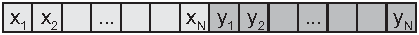
\includegraphics[draft=false,width=0.7\textwidth]{memory_layout2.pdf}}

\vspace{2ex}

\centerline{Everything seems easy!}
\vspace{2ex}
\centerline{{\bf But} how does {\tt ensemble} look like?}
 

\end{frame}




\begin{frame}[fragile]

 \heading{Ensemble of nonlinear pendulums}

 \begin{lstlisting}[basicstyle=\scriptsize\ttfamily]
struct ensemble
{
  const vector_type &m_eps;
  const vector_type &m_omega;
  double m_mu;

  ensemble(const vector_type &eps,const vector_type &omega,
    double mu)
      : m_eps(eps), m_omega(omega), m_mu(mu) { }

  void operator()(const state_type &x, state_type &dxdt,
    double t)
  {
    dxdt = std::make_tuple(
      x(1) ,
      -sin(x(0)) - m_mu*x(1) + m_eps*sin(m_omega*t)
      );
  }
};
 \end{lstlisting}


\end{frame}


